\documentclass[final,3p]{elsarticle}

% \documentclass[preprint,12pt]{elsarticle}

%% Use the option review to obtain double line spacing
%% \documentclass[authoryear,preprint,review,12pt]{elsarticle}

%% Use the options 1p,twocolumn; 3p; 3p,twocolumn; 5p; or 5p,twocolumn
%% for a journal layout:
% \documentclass[final,1p,times]{elsarticle}
%% \documentclass[final,1p,times,twocolumn]{elsarticle}
% \documentclass[final,3p,times]{elsarticle}
%% \documentclass[final,3p,times,twocolumn]{elsarticle}
% \documentclass[final,5p,times]{elsarticle}
%% \documentclass[final,5p,times,twocolumn]{elsarticle}
\usepackage[portuguese]{babel}

%% For including figures, graphicx.sty has been loaded in
%% elsarticle.cls. If you prefer to use the old commands
%% please give \usepackage{epsfig}

%% The amssymb package provides various useful mathematical symbols
\usepackage{amssymb}
\usepackage{amsmath}
\usepackage{multirow}

\usepackage{pgfplots}
\pgfplotsset{compat=1.18}
\usepgfplotslibrary{statistics}
\usepackage{pgfplotstable}
\usepackage{caption}
\usepackage{subcaption}

\usepackage{placeins}
\usepackage{hyperref}
\numberwithin{equation}{section}

\usepackage{algorithm}
\usepackage[noEnd=true, indLines=true]{algpseudocodex}
\algrenewcommand\algorithmicrequire{\textbf{Entrada:}}
\algrenewcommand\algorithmicwhile{\textbf{Enquanto}}
\algrenewcommand\algorithmicrepeat{\textbf{Repete}}
\algrenewcommand\algorithmicuntil{\textbf{Até}}
\algrenewcommand\algorithmicif{\textbf{Se}}
\algrenewcommand\algorithmicthen{\textbf{então}}
\algrenewcommand\algorithmicelse{\textbf{Caso contrário}}
\algrenewcommand\algorithmicensure{\textbf{Objetivo:}}
\algrenewcommand\algorithmicreturn{\textbf{Retorna:}}
\algrenewcommand\algorithmicdo{\textbf{faça}}
\algrenewcommand\algorithmicforall{\textbf{Para todos}}
\algnewcommand{\LineComment}[1]{\State \(\triangleright\) \textcolor{black!50}{\emph{#1}}}

% \usepackage[fleqn]{nccmath}
% \usepackage{multicol}


%=========== Gloabal Tikz settings
% \pgfplotsset{compat=newest}
% \usetikzlibrary{math}
% \pgfplotsset{
%     height = 10cm,
%     width = 10cm,
%     tick pos = left,
%     legend style={at={(0.98,0.30)}, anchor=east},
%     legend cell align=left,
%     }
%  \pgfkeys{
%     /pgf/number format/.cd,
%     fixed,
%     precision = 1,
%     set thousands separator = {}
% }

%% The amsthm package provides extended theorem environments
%% \usepackage{amsthm}

%% The lineno packages adds line numbers. Start line numbering with
%% \begin{linenumbers}, end it with \end{linenumbers}. Or switch it on
%% for the whole article with \linenumbers.
%% \usepackage{lineno}

\usepackage{listings}
\usepackage{xcolor}

\definecolor{codegreen}{rgb}{0,0.6,0}
\definecolor{codegray}{rgb}{0.5,0.5,0.5}
\definecolor{codepurple}{rgb}{0.58,0,0.82}
\definecolor{backcolour}{rgb}{0.98,0.98,0.98}

\lstdefinestyle{mystyle}{
    backgroundcolor=\color{backcolour},
    commentstyle=\color{codegreen},
    keywordstyle=\color{magenta},
    numberstyle=\tiny\color{codegray},
    stringstyle=\color{codepurple},
    basicstyle=\ttfamily\footnotesize,
    breakatwhitespace=false,
    breaklines=true,
    captionpos=b,
    keepspaces=true,
    numbers=left,
    numbersep=5pt,
    showspaces=false,
    showstringspaces=false,
    showtabs=false,
    tabsize=2
}

\lstset{style=mystyle}

% \journal{Nuclear Physics B}

\begin{document}

\begin{frontmatter}

%% Title, authors and addresses

%% use the tnoteref command within \title for footnotes;
%% use the tnotetext command for theassociated footnote;
%% use the fnref command within \author or \address for footnotes;
%% use the fntext command for theassociated footnote;
%% use the corref command within \author for corresponding author footnotes;
%% use the cortext command for theassociated footnote;
%% use the ead command for the email address,
%% and the form \ead[url] for the home page:
%% \title{Title\tnoteref{label1}}
%% \tnotetext[label1]{}
%% \author{Name\corref{cor1}\fnref{label2}}
%% \ead{email address}
%% \ead[url]{home page}
%% \fntext[label2]{}
%% \cortext[cor1]{}
%% \affiliation{organization={},
%%             addressline={},
%%             city={},
%%             postcode={},
%%             state={},
%%             country={}}
%% \fntext[label3]{}

\title{Estimativa do Ponto de Operação de um Sistema de Produção Simples\tnoteref{label_title}}
\tnotetext[label_title]{Relatório número 1 como parte dos requisitos da disciplina PP590: Tópicos em Geoengenharia de Reservatórios.}

%% use optional labels to link authors explicitly to addresses:
%% \author[label1,label2]{}
%% \affiliation[label1]{organization={},
%%             addressline={},
%%             city={},
%%             postcode={},
%%             state={},
%%             country={}}
%%
%% \affiliation[label2]{organization={},
%%             addressline={},
%%             city={},
%%             postcode={},
%%             state={},
%%             country={}}

\author{Tiago C. A. Amorim\fnref{label_author}}
\tnotetext[label_author]{Atualmente cursando doutorado no Departamento de Engenharia de Petróleo da Faculdade de Engenharia Mecânica da UNICAMP (Campinas/SP, Brasil).}
\ead{t100675@dac.unicamp.br}
\affiliation[Tiago C. A. Amorim]{organization={Petrobras},%Department and Organization
addressline={Av. Henrique Valadares, 28},
city={Rio de Janeiro},
postcode={20231-030},
state={RJ},
country={Brasil}}

\begin{abstract}
    Foi desenvolvido em Python um sistema para realizar a estimativa da perda de carga ao longo de um poço produtor satélite. Os testes realizados mostraram que, para as condições avaliadas, é possível conseguir bons resultados com poucas subdivisões dos elementos descritos.
\end{abstract}


%%Graphical abstract
% \begin{graphicalabstract}
%\includegraphics{grabs}
% \end{graphicalabstract}

%%Research highlights
% \begin{highlights}
% \item Research highlight 1
% \item Research highlight 2
% \end{highlights}

\begin{keyword}
    Modelo integrado \sep Correlações Black-Oil
%% keywords here, in the form: keyword \sep keyword

%% PACS codes here, in the form: \PACS code \sep code

%% MSC codes here, in the form: \MSC code \sep code
%% or \MSC[2008] code \sep code (2000 is the default)

\end{keyword}

\end{frontmatter}

%% \linenumbers

%% main text
\section{Introdução}

    Este relatório descreve os principais elementos desenvolvidos para resolver o exercício número 1 proposto na 1$^a$ aula de Tópicos em Geoengenharia de Reservatórios.

\section{Metodologia}

    \subsection{Problema Proposto}

        Foi proposto encontrar o ponto de operação de um poço produtor de óleo conectado diretamente a uma unidade de produção (configuração \emph{satélite}). Pela descrição na figura \ref{fig:problema_proposto} observa-se que:

        \begin{itemize}
            \item O problema é isotérmico: serão ignoradas as trocas térmicas na formulação.
            \item O óleo é muito subsaturado: todas as equações desenvolvidas irão considerar que não existe gás livre ao longo da tubulação.
        \end{itemize}

        \begin{figure}
            \centering
            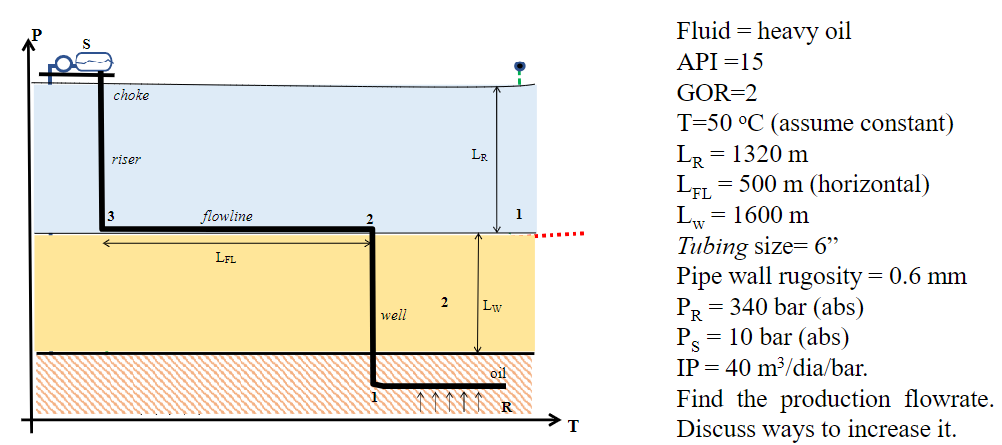
\includegraphics[width=0.8\textwidth]{Problem_01.png}
            \caption{Problema proposto número 1.}
            \label{fig:problema_proposto}
        \end{figure}

        Toda a resolução do problema foi feita em \texttt{Python}. Foram criados módulos específicos para cada elemento integrante do problema proposto. Dentro de cada módulo um ou mais objetos foram construídos. O código mais atual pode ser encontrado em \href{https://github.com/TiagoCAAmorim/IntegratedModel/tree/main/sample}{https://github.com/TiagoCAAmorim/IntegratedModel}.

    \subsection{Correlações Black-Oil \emph{(Módulo \texttt{pvt.py})}}

        Para este problema todas a propriedades de óleo foram estimadas a partir de correlações \emph{clássicas}:

        \begin{itemize}
            \item Pressão de bolha, fator volume de formação do óleo na pressão de bolha e viscosidade por Standing \cite{standing1952volumetric}.
            \item Compressibilidade do óleo na pressão de bolha por Vasquez e Beggs \cite{VasquezBeggs}.
        \end{itemize}

        Não foram necessárias para resolver o problema proposto, mas também foram implementadas correlações para cálculo de propriedades de gás com correlações de Standing (z e Bg).

        Dentro do módulo \texttt{pvt.py} existe a descrição de uma classe: \textbf{PVT}. O usuário precisa informar algumas informações básicas (api, pressão, temperatura, dg etc.) e pode usar as rotinas desenvolvidas para calcular outras propriedades com as correlações. Observou-se que existe um desvio entre a correlação de Standing para pressão de bolha e a inversão da correlação de razão de solubilidade (figura \ref{fig:pb}). Para manter coerência entre as diferentes estimativas, optou-se por utilizar no cálculo da pressão de boha a fórmula invertida a partir da correlação de razão de solubilidade. O usuário ainda tem acesso à correlação original de Standing.

        \begin{figure}
            \centering
            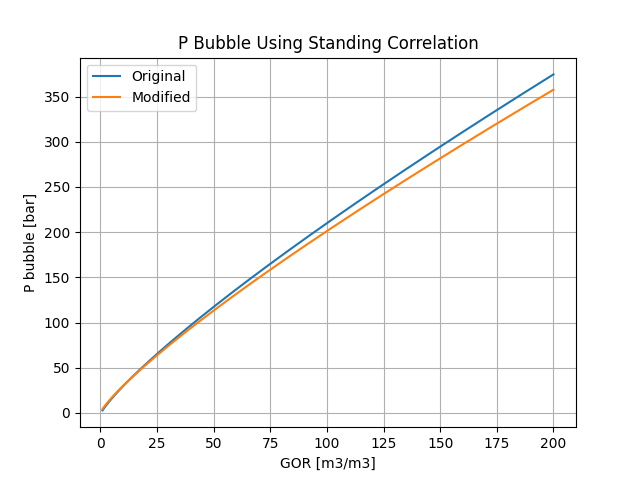
\includegraphics[width=0.6\textwidth]{pvt/p_bubble.png}
            \caption{Pressão de bolha pela correlação de Standing (\emph{Original}) e invertendo a correlação de razão de solubilidade de Standing (\emph{Modified}).}
            \label{fig:pb}
        \end{figure}

        Para o problema proposto é informado um fluido de baixa razão gás-óleo. Como a pressão de bolha deste fluido (11.83 bar a 50$^o$C) é muito próxima da menor pressão do sistema a ser modelado (10 bar), será possível ter uma boa estimativa considerando apenas óleo no sistema. Um problema que aparece é o do comportamento do fator volume de formação ($Bo$), pois o fluido estará submetido a uma pressão muito maior que a sua pressão de bolha. Usualmente é suficiente usar a aproximação linear para calcular o $Bo$ de um óleo subsaturado (equação \ref{eq:bo_linear}). Foi avaliado o efeito de considerar a forma \emph{exponencial} no cálculo do $Bo$ (equação \ref{eq:bo_exponencial}). Observa-se que para o fluido do problema proposto existe uma diferenciando não desprezível no $Bo$ em função da formulação utilizada (figura \ref{fig:bo_problema_proposto}). Optou-se por utilizar a forma \emph{exponencial} por padrão em todos os cálculos.

        \begin{align}
          B_o &= B_{ob} [1 + c_{ob}(p_b-p)] \label{eq:bo_linear} \\
          B_o &= B_{ob} e^{c_{ob}(p_b-p)} \label{eq:bo_exponencial}
        \end{align}

        \begin{figure}
            \centering
            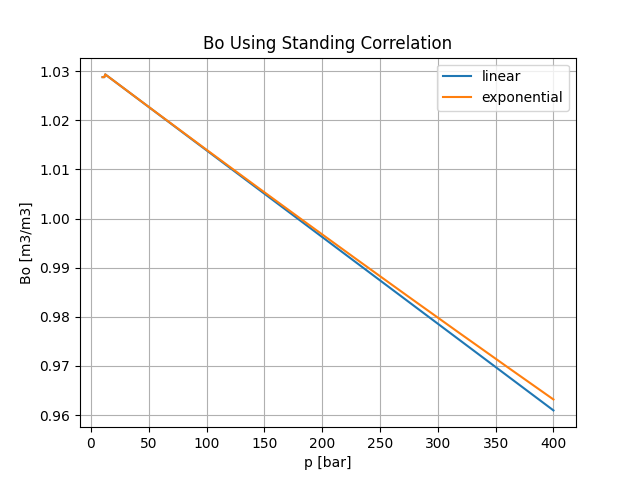
\includegraphics[width=0.6\textwidth]{pvt/bo2.png}
            \caption{Estimativa de fator volume de formação para o fluido do problema proposto.}
            \label{fig:bo_problema_proposto}
        \end{figure}

        Todos os testes realizados com as funcionalidades implementadas estão no arquivo \texttt{pvt\_tests.py}.

    \subsection{Índice de Produtividade \emph{(Módulo \texttt{ipr.py})}}

        Para este problema o modelo de reservatório será substituído por um índice de produtividade ($40\,m^3/d/bar$). Assumiu-se que esta medida segue a prática mais usual de que a vazão de óleo está em condições padrão.

        Neste módulo está descrito apenas uma classe: \textbf{IPR}. O usuário precisa fornecer a pressão média do reservatório e o valor do índice de produtividade. Uma função retorna a vazão, em condições padrão, em função da pressão de fundo ($p_{wf}$).

        Foi implementada uma função para estimativa do índice de produtividade a partir de parâmetros de reservatório. Foram implementadas duas variações do cálculo do índice de produtividade \cite{rosa2006engenharia}: fluxo pseudopermanente (equação \ref{eq:ip_pseudoperm}) e fluxo permanente (equação \ref{eq:ip_perm}).

        \begin{align}
          IP_{pseudoperm} [m^3/d/bar] &= \frac{k[mD] \, h[m]}{18.662 \, B_o \, \mu[cP]} \frac{1}{\left[ ln(\frac{r_e}{r_w}) - \frac{3}{4} + S \right] } \label{eq:ip_pseudoperm} \\
          IP_{permanente} [m^3/d/bar] &= \frac{k[mD] \, h[m]}{18.662 \, B_o \, \mu[cP]} \frac{1}{\left[ ln(\frac{r_e}{r_w}) - \frac{1}{2} + S \right] } \label{eq:ip_perm}
        \end{align}

        \subsection{Equações de Balanço \emph{(Módulo \texttt{flow.py})}}

        Neste módulo foram definidas três classes de objetos:

        \begin{itemize}
          \item \texttt{SubFlowElement}: Classe onde são feitos os cálculos de balanço. Tem rotinas para cálculo de $(p,T,Q)$ na saída do elemento em função de $(p,T,Q)$ na entrada. E vice-versa.
          \item \texttt{FlowElement}: Classe que tem uma coleção de \texttt{SubFlowElement}. O usuário define um elemento linear (riser, flow etc.), suas propriedades (diâmetro, rugosidade, PVT etc.) e a sua discretização. Uma rotina de cálculo faz os cálculos de balanço dividindo o elmento em vários \texttt{SubFlowElement}.
          \item \texttt{CompositeFlowElement}: Classe que contém uma coleção de \texttt{FlowElement}. Nesta classe o usuário define vários elementos lineares conectados entre si, com todas as suas propriedades. A rotina realiza os cálculos de balanço utilizando os \texttt{FlowElement}. A ordem dos elementos segue a direção do fluxo. Também é possível definir uma IPR e fazer os cálculos do ponto de operação com o método da secante \cite{burden2016analise}.
        \end{itemize}

        Para resolver o problema proposto foram implementadas rotinas de cálculo do balanço de massa (equação \ref{eq:balanco_massa}) e do balanço de energia mecânica (equação \ref{eq:balanco_mecanico}). O termo de ganho associado a turbomáquinas não foi implementado ($H_{tm}$). Como o problema proposto é isotérmico, o balanço de energia térmica não foi implementado.

        Todos os cálculos são feitos por elemento linear, avaliando os termos das equações na entrada ($in$) e na saída ($out$). Apenas o termo $\overline{\rho}$ é avaliado na pressão \emph{média} do elemento ($\frac{p_{in}+p_{out}}{2}$). Como a pressão \emph{média} depende de ambas pressões de entrada e saída, é feito um processo iterativo para chegar ao resultado.

        \begin{align}
          \frac{dm}{dt} &= \dot{m}  = \rho_{in} V_{in} A_{in} = \rho_{out} V_{out} A_{out} \label{eq:balanco_massa} \\
          p_{in} - p_{out} &= \overline{\rho} g \left[ (z_{out} - z_{in}) + H_L - H_{tm} + \frac{V_{out}^2 - V_{in}^2}{2g} \right] \label{eq:balanco_mecanico}
        \end{align}

        A perda de carga devido à fricção (equação \ref{eq:hloss}) é calculada com o fator de fricção da fórmula da Hall (equação \ref{eq:ff}). O termo $V$ da equação \ref{eq:hloss} é avaliado na pressão \emph{média} do elemento.

        \begin{align}
          Re &= \frac{4 \, \dot{m}}{\pi \, \mu \, D} \label{eq:reynolds} \\
          f &=
          \begin{cases}
            \frac{64}{Re} & \text{se } Re < 2300 \\
            0.0055 \left[ 1+ \sqrt[3]{2.\,10^4 \frac{\varepsilon}{D} + \frac{10^6}{Re}}   \right]     & \text{se } Re \geq 2300
        \end{cases} \label{eq:ff} \\
          H_L &= f \frac{L \, V^2}{D \, 2g} \label{eq:hloss}
        \end{align}

        Todos os testes realizados com as funcionalidades implementadas estão no arquivo \texttt{flow\_tests.py}.

\section{Resultados}

        Foram criados diferentes testes para avaliar a qualidade dos resultados das rotinas implementadas:

        \begin{itemize}
          \item Em geral os testes foram feitos nas \emph{duas direções}, isto é, informando $(p,T,Q)$ na entrada e calculando os valores de saída, e também o inverso. Desta forma foi possível avaliar a estabilidade das rotinas. Em todos os testes os valores mantiveram concordância.
          \item Para o fluido do problema proposto a queda de pressão no trecho horizontal se mostrou bem pequena (figura \ref{fig:linha_horizontal}).
          \item O cálculo da pressão de saída de uma linha vertical se mostrou pouco sensível ao número de subdivisões do elemento (figura \ref{fig:linha_vertical}). Menos de 100 elementos foram suficientes para estimar a pressão de saída.
        \end{itemize}

        \begin{figure}
          \centering
          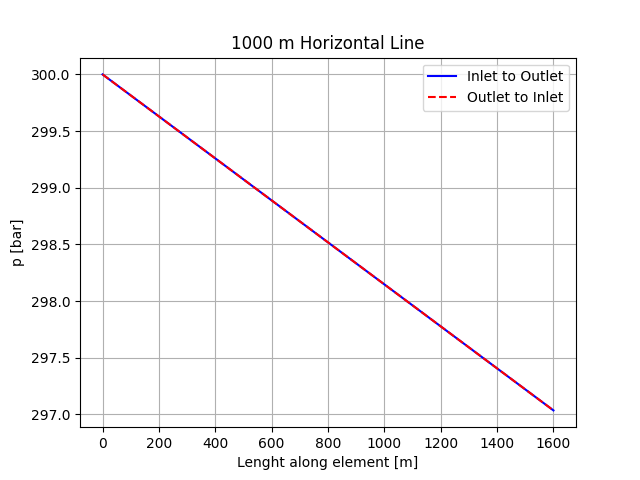
\includegraphics[width=0.6\textwidth]{flow/horizontal.png}
          \caption{Estimativa de fator volume de formação para o fluido do problema proposto.}
          \label{fig:linha_horizontal}
        \end{figure}

        \begin{figure}
          \centering
          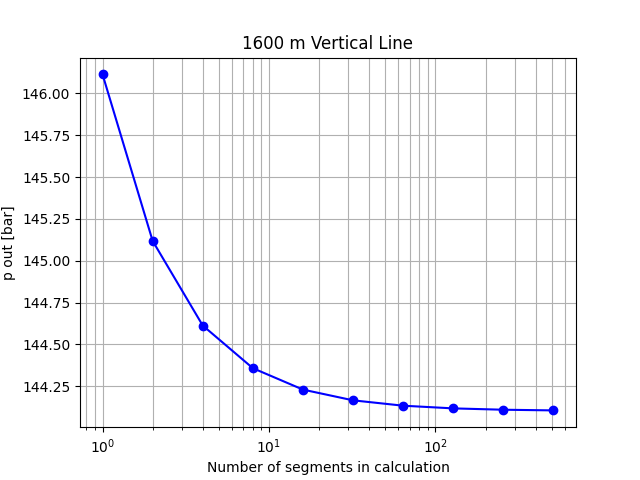
\includegraphics[width=0.6\textwidth]{flow/vertical_sensibility.png}
          \caption{Estimativa de fator volume de formação para o fluido do problema proposto.}
          \label{fig:linha_vertical}
        \end{figure}

        Para o cálculo do problema proposto os elementos foram subdivididos de forma a terem \emph{subelementos} de 10 m de comprimento nos trechos verticais e de 100 m no trecho horizontal. O ponto de operação encontrado foi em $p_{wf} = 295.565 \,bar$ e $q = 1777.4 \, m^3 std/d$ (figura \ref{fig:operacao}). Como antecipado, o trecho em que o sistema pode ter gás livre é muito curto, de forma que a implementação proposta em que se considera apenas óleo é suficiente (figura \ref{fig:pressao}). Diversos resultados são mostrados nas figuras \ref{fig:resultados}.

        \begin{figure}
          \centering
          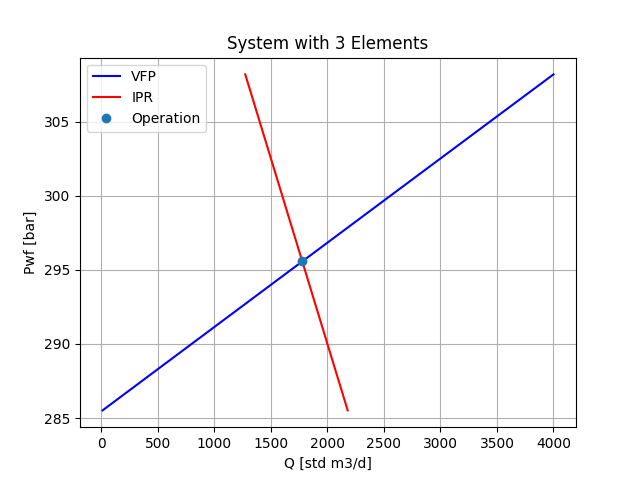
\includegraphics[width=0.6\textwidth]{flow/system1_qp.png}
          \caption{Ponto de operação do problema proposto.}
          \label{fig:operacao}
        \end{figure}

        \begin{figure}
          \centering
          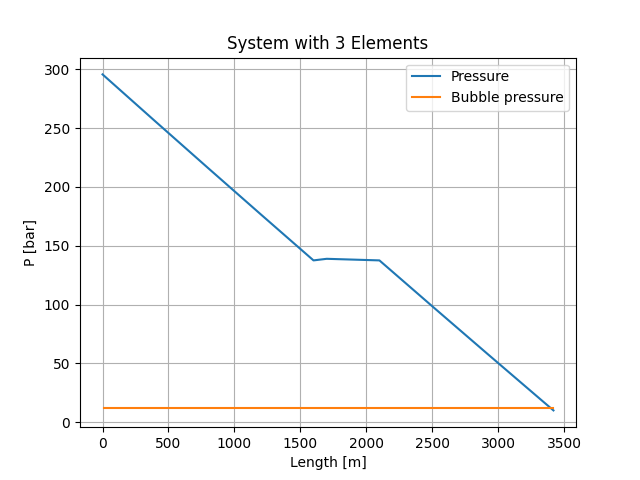
\includegraphics[width=0.6\textwidth]{flow/system1_operation.png}
          \caption{Pressão ao longo dos elementos do problema proposto.}
          \label{fig:pressao}
        \end{figure}


        \begin{figure}
          \centering

          \begin{subfigure}{0.45\textwidth}
            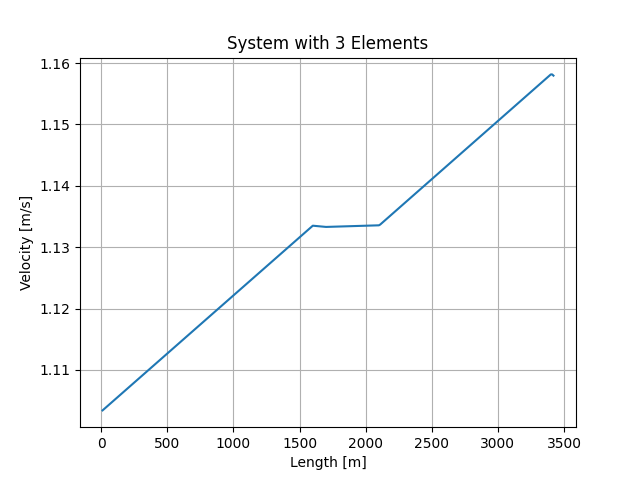
\includegraphics[width=\textwidth]{flow/system1_v.png}
            \caption{Velocidade}
          \end{subfigure}
          \hfill
          \begin{subfigure}{0.45\textwidth}
            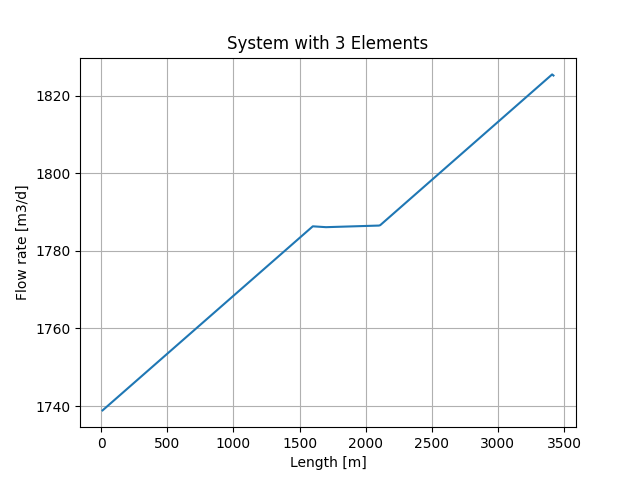
\includegraphics[width=\textwidth]{flow/system1_q.png}
            \caption{Vazão}
          \end{subfigure}

          \begin{subfigure}{0.45\textwidth}
            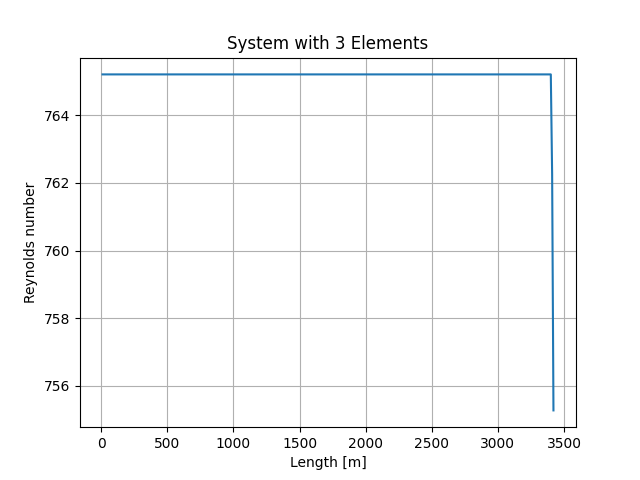
\includegraphics[width=\textwidth]{flow/system1_Re.png}
            \caption{Número de Reynolds}
          \end{subfigure}
          \hfill
          \begin{subfigure}{0.45\textwidth}
            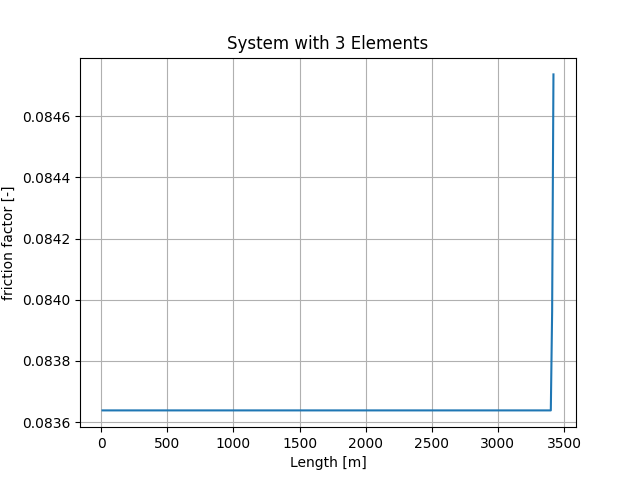
\includegraphics[width=\textwidth]{flow/system1_f.png}
            \caption{Fator de fricção}
          \end{subfigure}

          \begin{subfigure}{0.45\textwidth}
            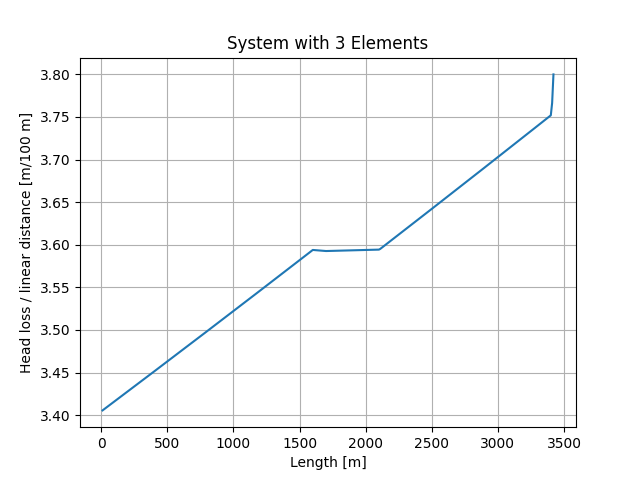
\includegraphics[width=\textwidth]{flow/system1_hl.png}
            \caption{Perda de carga por comprimento linear}
          \end{subfigure}
          \hfill
          \begin{subfigure}{0.45\textwidth}
            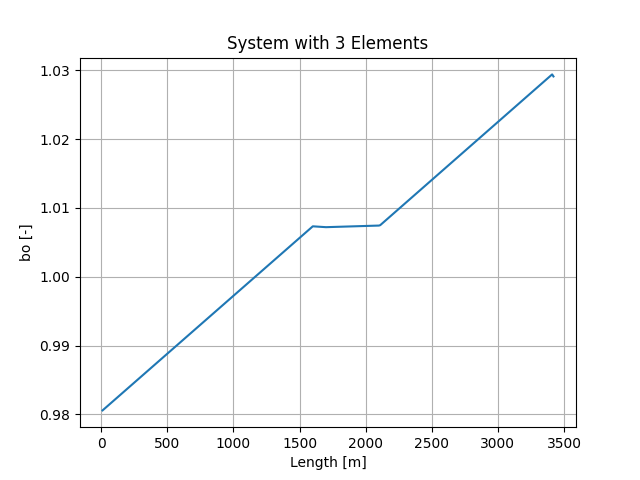
\includegraphics[width=\textwidth]{flow/system1_bo.png}
            \caption{Fator volume de formação}
          \end{subfigure}

          \caption{Principais resultados ao longo dos elementos do problema proposto.}
          \label{fig:resultados}
        \end{figure}

        Foram feitas algumas sensibilidades do ponto de operação com variáveis do problema: pressão de chegada e diâmetro da tubulação (figuras \ref{fig:sensibilidade}). A pressão de chegada apresentou uma correlação linear com a vazão do ponto de operação do sistema. A sensibilidade do diâmetro mostrou uma relação menos que linear com a vazão.

        \begin{figure}
          \centering

          \begin{subfigure}{0.45\textwidth}
            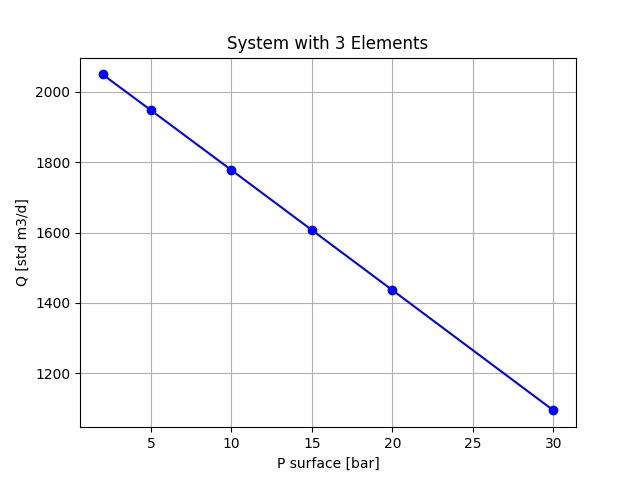
\includegraphics[width=\textwidth]{flow/system1_p_out.png}
            \caption{Pressão de chegada}
          \end{subfigure}
          \hfill
          \begin{subfigure}{0.45\textwidth}
            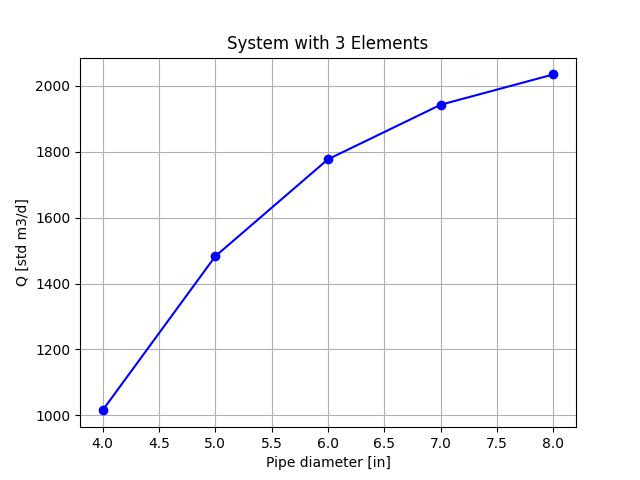
\includegraphics[width=\textwidth]{flow/system1_d.png}
            \caption{Diâmetro da tubulação}
          \end{subfigure}

          \caption{Sensibilidade do problema proposto.}
          \label{fig:sensibilidade}
        \end{figure}

\section{Conclusão}

        O problema proposto mostrou um comportamento aparentemente linear com os dados de entrada. Como trata-se da simulação do fluxo de um fluido monofásico, isotérmico e em regime laminar, este comportamento já era esperado. O sistema desenvolvido mostrou que para o problema proposto não há necessidade de fazer muitas subdivisões nos elementos lineares.


%% The Appendices part is started with the command \appendix;
%% appendix sections are then done as normal sections

\appendix

%% \section{}
%% \label{}

%% If you have bibdatabase file and want bibtex to generate the
%% bibitems, please use
%%

\bibliographystyle{elsarticle-num}
\bibliography{refs}

%% else use the following coding to input the bibitems directly in the
%% TeX file.

% \begin{thebibliography}{00}

%% \bibitem{label}
%% Text of bibliographic item

% \bibitem{}

% \end{thebibliography}


\end{document}
\endinput